\documentclass{article}
\usepackage[T1]{fontenc}
\usepackage{lmodern}
\usepackage{graphicx}
\usepackage{amsmath,amssymb}
\usepackage[a4paper,margin=2cm]{geometry}
\usepackage[absolute,overlay]{textpos}
\setlength{\TPHorizModule}{1mm}
\setlength{\TPVertModule}{1mm}
\usepackage[indonesian]{babel}
\usepackage{hyperref}
\setlength{\emergencystretch}{2em}
% unit: Halaman 25

\begin{document}

% === Halaman 25 (llm) ===

\vspace{138.11mm}

\begin{itemize}
    \item $P(B)$ merupakan luaran dari fungsi $f$.
    \item Bit-bit $P(B)$ di-XOR-kan dengan $L_{i-1}$ menghasilkan $R_i$:
    \[ R_i = L_{i-1} \oplus P(B) \]
    \item Jadi, luaran dari putaran ke-$i$ adalah
    \[ (L_i, R_i) = (R_{i-1}, L_{i-1} \oplus P(B)) \]
\end{itemize}
\vspace{10mm}

% deskripsi: Diagram alur logika yang menunjukkan operasi XOR antara input L_{i-1} (32 bit) dan output fungsi f untuk menghasilkan R_i (32 bit).
% bbox normalisasi: [0.4630, 0.4180, 0.9330, 0.8830]
\begin{textblock*}{98.70mm}(97.23mm,124.15mm)
\noindent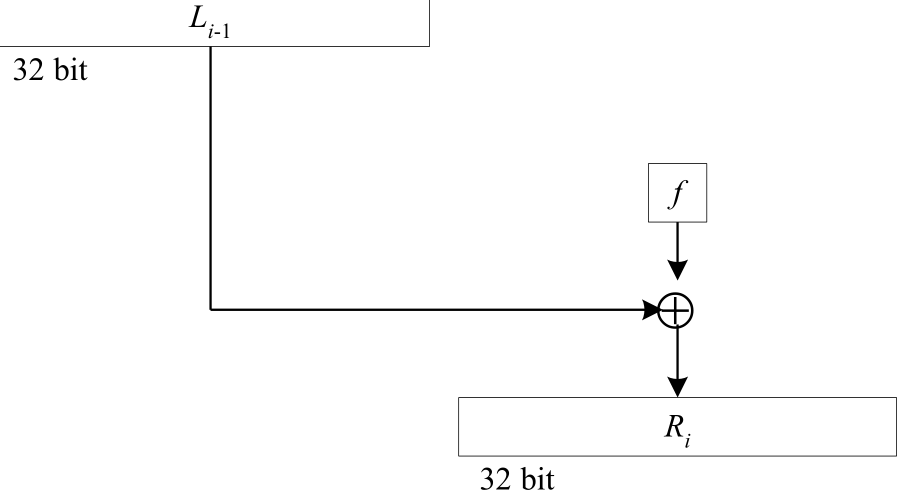
\includegraphics[width=98.70mm,height=138.11mm]{../../images/llm/page_025_img_01.png}%
\end{textblock*}

\end{document}
